\documentclass[9pt]{article}
\usepackage{enumitem}
\usepackage{latexsym}
\usepackage{amsfonts}
\usepackage{float}
\usepackage{fullpage}
\usepackage{graphicx}
\usepackage{geometry}
\usepackage{pdflscape}
\usepackage{booktabs}
\usepackage{listings}
\usepackage{float}
\usepackage{subfigure}
\usepackage{amsmath} % Add the necessary package for the control sequence
\usepackage{setspace} % Add the necessary package for adjusting line spacing
\usepackage{hyperref}
% \usepackage{subcaption}
\geometry{
    left=0.5in,
    right=0.5in,
    top=0.5in,
    bottom=0.5in
}
\newcommand{\N}{\mathcal{N}}
\newcommand{\R}{\mathcal{R}}
\newcommand{\A}{\mathcal{A}}

\newcommand{\handout}[4]{
   \renewcommand{\thepage}{#1-\arabic{page}}
   \pagestyle{empty}
   \noindent
   \begin{center}
   \framebox{
      \vbox{
    \hbox to 6in { {\bf CS657}
         \hfill #2 }
       \vspace{4mm}
       \hbox to 6in { {\Large \hfill #4  \hfill} }
       \vspace{2mm}
       \hbox to 5.78in { {\it #3 \hfill} }
      }
   }
   \end{center}
   \vspace*{4mm}
}

\newcommand{\solheader}[2]{\handout{#1}{\today}{#2}{HW2:Predicting Fake Job Posting}}


%\input{sol_preamble.tex}

% topics: Turing machines, universal TMs, languages, TMs deciding a language, uncomputable languages

\begin{document}
%%%%%%% Edit this next line: parameter 1 is the homework number, the 2nd is your name.
\solheader{1}{Antara Tewary (G01413546),Ankit Kumar (G01436204)}

\begin{enumerate}
    \item \textbf{\underline{Introduction}}\\
    This assignment aims to create a system that flags suspicious job postings on Indeed.com, addressing the challenge of fraudulent postings that mislead the efforts of job seekers. We are using Fake Job Prediction Dataset, which contains 18000 job descriptions out of which 800 are fraudulent samples. The goal is to create an automated model which prioritizes which posting to review based on the likelihood of it being fraudulent.
    
    \item \textbf{\underline{Data Preparation}} 
    \begin{itemize}
      \item \textit{Label Encoding and Filtering Invalid Data}: The target column fraudulent was cast to integer type to represent legitimate (0) and fake (1) job postings. Any records with invalid values were filtered out.
      \item \textit{Handling Missing Values}:We identified missing values by calculating percentage of null or NaN values across columns and dropped those with more than 1\% null values to reduce noise.
      \item \textit{Text Cleaning}: The job descriptions were cleaned by removing special characters, converting text to lowercase, and removing stop words to ensure uniformity.
      \item \textit{Balancing the Dataset}:To address class imbalance, we undersampled the majority class (legitimate postings) to match the minority class (fake postings), ensuring balanced data for model training. We used sampleBy function in PySpark to match the number of legitimate postings to the number of fraudulent postings. Balancing the dataset removes the risk of bias towards majority class during model training.
    \end{itemize}
    Here are some statistics of the dataset after cleaning:
    \begin{figure}[H]
      \centering
      \subfigure[Class distribution before and after balancing]{
        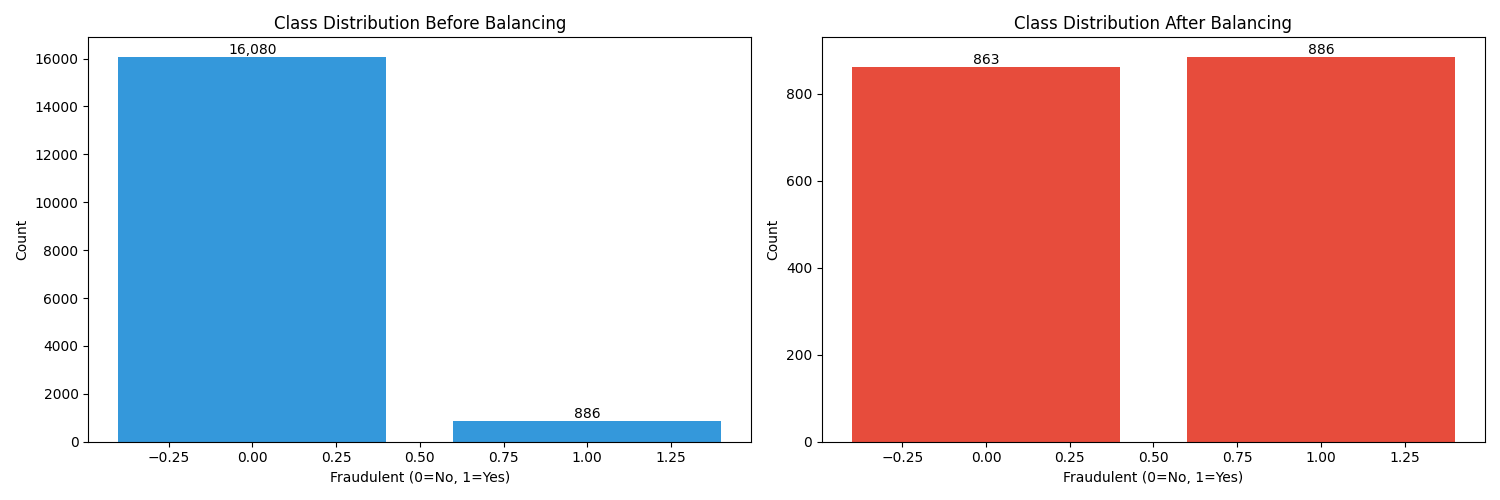
\includegraphics[width=0.47\textwidth]{class_distribution.png}
        \label{fig:class_distribution}
      }
      \hspace{0.02\textwidth}
      \subfigure[The effect of text cleaning by comparing text length distributions before and after cleaning.]{
          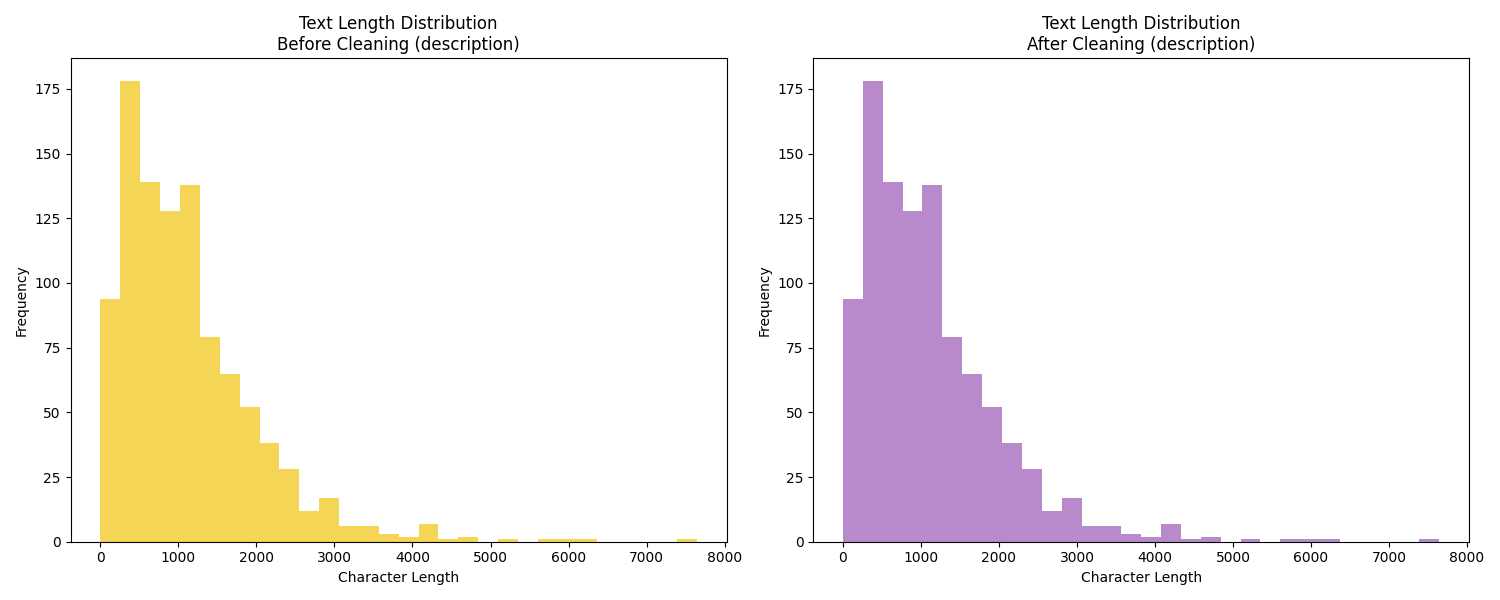
\includegraphics[width=0.47\textwidth]{text_cleaning_effects.png}
          \label{fig:text-cleaning-effects}
      }
      \hspace{0.02\textwidth}
      \subfigure[\% of missing values for each column]{
          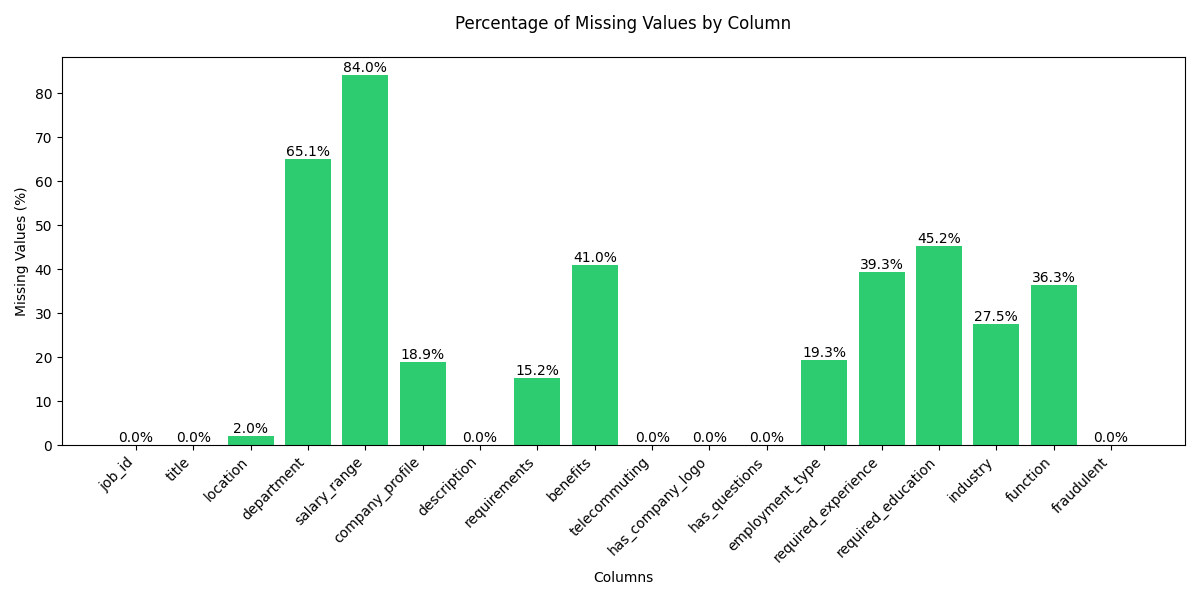
\includegraphics[width=0.58\textwidth]{missing_values.png}
          \label{fig:missing-values-plot}
      }
      \hspace{0.02\textwidth}      
      \caption{Data Preparation Statistics}
      \label{fig:data_statistics_combined}
  \end{figure}
  \item \textbf{\underline{Feature Engineering}}\\ 
  
\end{enumerate}

\end{document}
